\documentclass{standalone}
\usepackage{tikz}
\usepackage{ctex,siunitx}
\setCJKmainfont{Noto Serif CJK SC}
\usepackage{tkz-euclide}
\usepackage{amsmath}
\usetikzlibrary{patterns, calc}
\usetikzlibrary {decorations.pathmorphing, decorations.pathreplacing, decorations.shapes,}

\begin{document}
\small
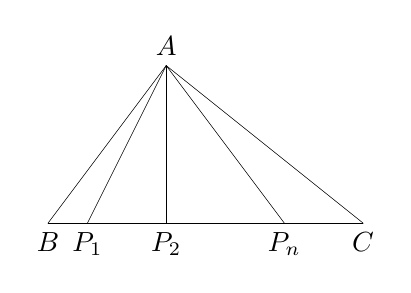
\begin{tikzpicture}[>=stealth,scale=1]
  \tkzSetUpPoint[fill=black]
  % \useasboundingbox(-1,-0.75)rectangle(3.7,1.4);
  \tkzDefPoints{0/0/B, .5/0/P_1,1.5/0/P_2,3/0/P_n, 4/0/C, 1.5/2/A}
	\tkzLabelPoints[below](P_1,P_2,P_n,B,C)	
	\tkzDrawSegments(A,B A,P_1 A,P_2 A,P_n A,C B,C)
	\tkzLabelPoints[above](A)	
\end{tikzpicture}
\end{document}